% ========================================
%	Header einbinden
% ========================================

\documentclass[bibtotoc,titlepage]{scrartcl}

% Deutsche Spracheinstellungen
\usepackage[ngerman,german]{babel, varioref}
\usepackage[T1]{fontenc}
\usepackage[utf8]{inputenc}

%\usepackage{marvosym}

\usepackage{amsfonts}
\usepackage{amssymb}
\usepackage{amsmath}
\usepackage{amscd}
\usepackage{amstext}

\usepackage{longtable}

%\usepackage{bibgerm}

\usepackage{footnpag}

\usepackage{ifthen}                 %%% package for conditionals in TeX
\usepackage[amssymb]{SIunits}
%Für textumflossene Bilder und Tablellen
%\usepackage{floatflt} - veraltet

%Für Testzwecke aktivieren, zeigt labels und refs im Text an.
%\usepackage{showkeys}

% Abstand zwischen zwei Absätzen nach DIN (1,5 Zeilen)
% \setlength{\parskip}{1.5ex plus0.5ex minus0.5ex}

% Einrückung am Anfang eines neuen Absatzes nach DIN (keine)
%\setlength{\parindent}{0pt}

% Ränder definieren
% \setlength{\oddsidemargin}{0.3cm}
% \setlength{\textwidth}{15.6cm}

% bessere Bildunterschriften
%\usepackage[center]{caption2}


% Problemlösungen beim Umgang mit Gleitumgebungen
\usepackage{float}

% Nummeriert bis zur Strukturstufe 3 (also <section>, <subsection> und <subsubsection>)
%\setcounter{secnumdepth}{3}

% Führt das Inhaltsverzeichnis bis zur Strukturstufe 3
%\setcounter{tocdepth}{3}
\usepackage[version=3]{mhchem}
	\mhchemoptions{minus-sidebearing-left=0.06em, minus-sidebearing-right=0.11em}
\usepackage{exscale}

\newenvironment{dsm} {\begin{displaymath}} {\end{displaymath}}
\newenvironment{vars} {\begin{center}\scriptsize} {\normalsize \end{center}}


\newcommand {\en} {\varepsilon_0}               % Epsilon-Null aus der Elektrodynamik
\newcommand {\lap} {\; \mathbf{\Delta}}         % Laplace-Operator
\newcommand {\R} { \mathbb{R} }                 % Menge der reellen Zahlen
\newcommand {\e} { \ \mathbf{e} }               % Eulersche Zahl
\renewcommand {\i} { \mathbf{i} }               % komplexe Zahl i
\newcommand {\N} { \mathbb{N} }                 % Menge der nat. Zahlen
\newcommand {\C} { \mathbb{C} }                 % Menge der kompl. Zahlen
\newcommand {\Z} { \mathbb{Z} }                 % Menge der kompl. Zahlen
\newcommand {\limi}[1]{\lim_{#1 \rightarrow \infty}} % Limes unendlich
\newcommand {\sumi}[1]{\sum_{#1=0}^\infty}
\newcommand {\rot} {\; \mathrm{rot} \,}         % Rotation
\newcommand {\grad} {\; \mathrm{grad} \,}       % Gradient
\newcommand {\dive} {\; \mathrm{div} \,}        % Divergenz
\newcommand {\dx} {\; \mathrm{d} }              % Differential d
\newcommand {\cotanh} {\; \mathrm{cotanh} \,}   %Cotangenshyperbolicus
\newcommand {\asinh} {\; \mathrm{areasinh} \,}  %Area-Sinus-Hyp.
\newcommand {\acosh} {\; \mathrm{areacosh} \,}  %Area-Cosinus-H.
\newcommand {\atanh} {\; \mathrm{areatanh} \,}  %Area Tangens-H.
\newcommand {\acoth} {\; \mathrm{areacoth} \,}  % Area-cotangens
\newcommand {\Sp} {\; \mathrm{Sp} \,}
\newcommand {\mbe} {\stackrel{\text{!}}{=}}     %Must Be Equal
\newcommand{\qed} { \hfill $\square$\\}
\renewcommand{\i} {\imath}
\def\captionsngerman{\def\figurename{\textbf{Abb.}}}

%%%%%%%%%%%%%%%%%%%%%%%%%%%%%%%%%%%%%%%%%%%%%%%%%%%%%%%%%%%%%%%%%%%%%%%%%%%%
% SWITCH FOR PDFLATEX or LATEX
%%%%%%%%%%%%%%%%%%%%%%%%%%%%%%%%%%%%%%%%%%%%%%%%%%%%%%%%%%%%%%%%%%%%%%%%%%%%
%%%
\ifx\pdfoutput\undefined %%%%%%%%%%%%%%%%%%%%%%%%%%%%%%%%%%%%%%%%% LATEX %%%
%%%
\usepackage[dvips]{graphicx}       %%% graphics for dvips
\DeclareGraphicsExtensions{.eps,.ps}   %%% standard extension for included graphics
\usepackage[ps2pdf]{thumbpdf}      %%% thumbnails for ps2pdf
\usepackage[ps2pdf,                %%% hyper-references for ps2pdf
bookmarks=true,%                   %%% generate bookmarks ...
bookmarksnumbered=true,%           %%% ... with numbers
hypertexnames=false,%              %%% needed for correct links to figures !!!
breaklinks=true,%                  %%% breaks lines, but links are very small
linkbordercolor={0 0 1},%          %%% blue frames around links
pdfborder={0 0 112.0}]{hyperref}%  %%% border-width of frames
%                                      will be multiplied with 0.009 by ps2pdf
%
\hypersetup{ pdfauthor   = {Hannes Franke; Julius Tilly},
pdftitle    = {V301 Innenwiderstand und Leistungsanpassung}, pdfsubject  = {Protokoll FP}, pdfkeywords = {V301, Innenwiderstand, Leistungsanpassung},
pdfcreator  = {LaTeX with hyperref package}, pdfproducer = {dvips
+ ps2pdf} }
%%%
\else %%%%%%%%%%%%%%%%%%%%%%%%%%%%%%%%%%%%%%%%%%%%%%%%%%%%%%%%%% PDFLATEX %%%
%%%
\usepackage[pdftex]{graphicx}      %%% graphics for pdfLaTeX
\DeclareGraphicsExtensions{.pdf}   %%% standard extension for included graphics
\usepackage[pdftex]{thumbpdf}      %%% thumbnails for pdflatex
\usepackage[pdftex,                %%% hyper-references for pdflatex
bookmarks=true,%                   %%% generate bookmarks ...
bookmarksnumbered=true,%           %%% ... with numbers
hypertexnames=false,%              %%% needed for correct links to figures !!!
breaklinks=true,%                  %%% break links if exceeding a single line
linkbordercolor={0 0 1},
linktocpage]{hyperref} %%% blue frames around links
%                                  %%% pdfborder={0 0 1} is the default
\hypersetup{
pdftitle    = {V301 Innenwiderstand und Leistungsanpassung}, 
pdfsubject  = {Protokoll AP}, 
pdfkeywords = {V301, Innenwiderstand, Leistungsanpassung},
pdfsubject  = {Protokoll AP},
pdfkeywords = {V301, Innenwiderstand, Leistungsanpassung}}
%                                  %%% pdfcreator, pdfproducer,
%                                      and CreationDate are automatically set
%                                      by pdflatex !!!
\pdfadjustspacing=1                %%% force LaTeX-like character spacing
\usepackage{epstopdf}
%
\fi %%%%%%%%%%%%%%%%%%%%%%%%%%%%%%%%%%%%%%%%%%%%%%%%%%% END OF CONDITION %%%
%%%%%%%%%%%%%%%%%%%%%%%%%%%%%%%%%%%%%%%%%%%%%%%%%%%%%%%%%%%%%%%%%%%%%%%%%%%%
% seitliche Tabellen und Abbildungen
%\usepackage{rotating}
\usepackage{ae}
\usepackage{
  array,
  booktabs,
  dcolumn
}
\makeatletter 
  \renewenvironment{figure}[1][] {% 
    \ifthenelse{\equal{#1}{}}{% 
      \@float{figure} 
    }{% 
      \@float{figure}[#1]% 
    }% 
    \centering 
  }{% 
    \end@float 
  } 
  \makeatother 


  \makeatletter 
  \renewenvironment{table}[1][] {% 
    \ifthenelse{\equal{#1}{}}{% 
      \@float{table} 
    }{% 
      \@float{table}[#1]% 
    }% 
    \centering 
  }{% 
    \end@float 
  } 
  \makeatother 
%\usepackage{listings}
%\lstloadlanguages{[Visual]Basic}
%\allowdisplaybreaks[1]
%\usepackage{hycap}
%\usepackage{fancyunits}


% ========================================
%	Angaben für das Titelblatt
% ========================================

\title{Versuch 353 - Das Relaxationsverhalten eines RC-Kreises\\				% Titel des Versuchs 
\large TU Dortmund, Fakultät Physik\\ 
\normalsize Anfänger-Praktikum}

\author{Jan Adam\\			% Name Praktikumspartner A
{\small \href{jan.adam@tu-dortmund.de}{jan.adam@tu-dortmund.de}}	% Erzeugt interaktiven einen Link
\and						% um einen weiteren Author hinzuzfügen
Dimitrios Skodras\\					% Name Praktikumspartner B
{\small \href{dimitrios.skodras@tu-dortmund.de}{dimitrios.skodras@tu-dortmund.de}}		% Erzeugt interaktiven einen Link
}
\date{23.Oktober 2012}				% Das Datum der Versuchsdurchführung

% ========================================
%	Das Dokument beginnt
% ========================================

\begin{document}

% ========================================
%	Titelblatt erzeugen
% ========================================

\maketitle					% Jetzt wird die Titelseite erzeugt
\thispagestyle{empty} 				% Weder Kopfzeile noch Fußzeile

% ========================================
%	Der Vorspann
% ========================================

%\newpage					% Wenn Verzeichnisse auf einer neuen Seite beginnen sollen
%\pagestyle{empty}				% Weder Kopf- noch Fußzeile für Verzeichnisse

\tableofcontents

%\newpage					% eine neue Seite
%\thispagestyle{empty}				% Weder Kopf- noch Fußzeile für Verzeichnisse
%\listoffigures					% Abbildungsverzeichnis

%\newpage					% eine neue Seite
%\thispagestyle{empty}				% Weder Kopf- noch Fußzeile für Verzeichnisse
%\listoftables					% Tabellenverzeichnis
\newpage					% eine neue Seite


% ========================================
%	Kapitel
% ========================================

\section{Einleitung}				% Bei Bedarf

\section{Theorie}

Relaxation bezeichnet das Zurückkehren eines angeregten Systems in seinen Ruhezustand. Wird  beispielsweise ein stark gedämpftes Pendel ausgelenkt, so entsteht eine Rückstellkraft, die es wieder in seine Ruheposition zurückführt. Die asymptotische Annäherung, wird durch das Relaxationsverhalten beschrieben.\\
In diesem Versuch soll ein RC-Schwingkreis auf sein Relaxationsverhalten untersucht werden. Dieser besteht aus einem Kondensator mit der Kapazität C, der über einen Widerstand R mit einer Spannung $U_0$ auf- und entladen wird.\\
\begin{figure}[htbp]
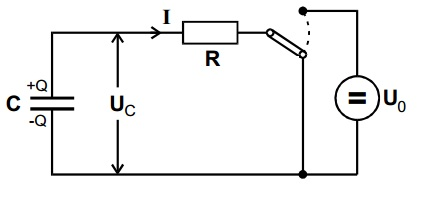
\includegraphics[width=8cm]{pics/aufbau.jpg}
\centering
\end{figure}

Mit Hilfe des Kirchhoffschen und Ohmschen Gesetztes lässt sich fürs Auf- und Entladen die folgende Differentialgleichung 
für dieses System herleiten:
\begin{align}
\dot Q(t)=-\frac{1}{RC} Q(t)
\end{align}

deren Lösungen folgende Exponentialfunktionen sind:
\begin{align}
Q(t)&=Q_0(1-e^{-\frac{1}{RC}t)}\\
Q(t)&=Q_0 e^{-\frac{1}{RC}t}
\end{align}

Der Exponent $-\frac{1}{RC}$ beschreibt dabei, wie schnell sich die Ladung des Kondensators ändert, bzw. wie schnell sich das System seinem Endzustand nähert. In folgender Tabelle ist die Zeit als Vielfaches der Konstante RC gegenüber dem relativen Anteil des Anfangswertes des Systems aufgetragen.
\begin{align*}
\begin{tabular}[t]{c|c|c|c|c|c}
Zeit in RC Einheiten 	&1 &2 &3 &4 &5\\ \hline
Restprozent 			&0,37 &0,14 &0,05 &0,02 &0,01\\
\end{tabular}
\end{align*}

RC ermöglicht es somit allgemein, qualitative Aussagen über relaxative Systeme zu treffen und wird deshalb auch als  Zeitkonstante $\tau$ des Relaxationsvorganges bezeichnet.\\

Zunächst wird das RC-Element mit einer relativ niederfrequenten ($\omega\ll\frac{1}{RC}$) Rechteckspannung $U_0$ betrieben. Die Frequenz wird so gewählt, damit sich der Kondensator bei jedem Phasendurchlauf immer noch vollständig auf- und entladen kann.
Im späteren Verlauf wird die Frequenz jedoch erhöht. Es bildet sich schließlich eine Phasenverschiebung 
\begin{align}
\varphi(\omega)=arctan(-\omega RC)
\label{varphi}
\end{align}

zwischen der Kondensatorspannung und der Generatorspannung heraus, da sich der Kondensator wegen des Widerstandes nicht instantan entladen kann.\\

Bei weiterer Erhöhung der Frequenz, ist die Dauer der Phase irgendwann nicht mehr lang genug, um den Kondensator vollständig zu entladen, bzw. ihn vollständig aufzuladen.
Die Amplitude der Kondensatorspannung erreicht dann nicht mehr den Maximalwert $U_0$ und hat keinen Nulldurchlauf mehr.
\begin{align}
A(\omega)= \frac{U_0}{\sqrt{1+\omega^2(RC)^2}}
\label{A_omega}
\end{align}
Gleichung \eqref{A_omega} beschreibt die reduzierte Amplitudenhöhe in Abhängigkeit von der Frequenz $\omega$.
Das RC-Glied behindert somit den Durchfluss des Wechselstroms bei höheren Frequenzen und wird deshalb auch als Tiefpass bezeichnet, da es Ströme mit langsamen Frequenzen ungehindert durchfließen lässt, während hochfrequente Signale abgemildert werden.\\

Bei hohen Frequenzen $\omega\gg\frac{1}{RC}$ arbeitet der RC-Kreis des weiteren als Integrator. Beliebige eingegebene Signale können am Kondensator in integrierter Form abgegriffen werden, ähnlich als würde man eine Funktion integrieren.
\begin{align}
U(t)=\frac{1}{RC} \int_0^t U(t')dt'
\label{int}
\end{align}

Gleichung \eqref{int} zeigt das Verhältnis zwischen der angelegten Wechselspannung U(t) und der am Kondensator abgegriffenen Spannung $U_c$. 
Wie man sehen kann, taucht wieder die Konstante $\frac{1}{RC}$ als charakteristische Größe auf. Diesmal ist sie der Proportionalitätsfaktor zwischen den beiden Spannungen.\\

\section{Durchführung}
\subsection{}
Zunächst soll die Zeitkonstante RC bestimmt werden. Hierzu erzeugt der Generator eine Rechteckspannung mit einer hinreichend kleinen Frequenz $\omega\ll\frac{1}{RC}$, damit der Kondensator noch vollständig auf- und entladen wird und zunächst vom Wechselstrom unbeeinflusst bleibt.
Zu verschiedenen Zeitpunkten wird während der Entladung die Kondensatorspannung $U_c$ gemessen und die Daten später halblogarithmisch aufgetragen. Die Steigung der sich ergebenden Geraden entspricht der Konstanten RC.

\subsection{}
Im nächsten Schritt wird der Schaltkreis mit einer Sinusspannung betrieben und die Frequenz $\omega$ schrittweise erhöht. Zu jeder Frequenz wird die Amplitude der Kondensatorspannung gemessen und alles als Graph dargestellt. Zu zeigen ist, dass bei höheren Frequenzen die Amplitude abnimmt, da die Phasendauer des Stroms zu kurz wird um den Kondensator noch vollständig aufzuladen, bzw. zu entladen. Desweiteren lässt sich mit Gleichung \eqref{A_omega} ebenfalls RC bestimmen. Die beiden Werte sollen anschließend miteinander verglichen und diskutiert werden.

\subsection{}
Der Versuch aus Teil b wird wiederholt, nur diesmal wird anstelle der Amplitude die Phasenverschiebung $\varphi$ gemessen und überprüft ob diese der Gleichung \eqref{varphi} genügt.

\subsection{}
Abschließend soll verifiziert werden, inwieweit das RC-Glied als Integrator arbeitet. Hierzu werden vom Generator nacheinander eine Sinus-, Dreieck-, und zwei verschiedene Rechteckspannungen erzeugt. 
Für die erfolgreiche Integration wird eine entsprechend hohe Frequenz gewählt und die erzeugten Graphen werden übereinander aufgetragen. Anschließend kann man beide miteinander vergleichen und qualitativ auswerten.

\section{Auswertung}
Hauptbetrachtungspunkt dieses Experiments ist die Bestimmung der Zeitkonstanten des bereitgestellten RC-Gliedes nach verschiedenen Methoden

\subsection{Auf- und Entladung des Kondensators}
Nach dem oben aufgeführten Schaltbild wurde das RC-Glied aufgebaut. Es wurde mit einer niederfrequenten Rechtecksspannung betrieben.
Dadurch wird der Kondensator über eine halbe Periode aufgeladen und danach entladen. Die Frequenz hierbei beträgt f = 42 Hz und die Ladespannung
U = 5V. Der in der folgenden Abbildung dargestellter exponentielle Abfall entspricht der Entladekurve des Kondensators.


\begin{figure}[htbp]
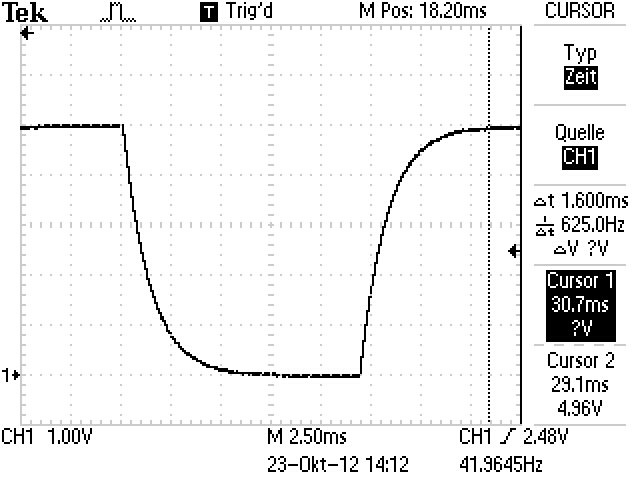
\includegraphics[width=8cm] {pics/TEK0000.JPG}
\centering
\end{figure}


Um die Zeitkonstante RC zu ermitteln wird zu vielen Zeiten (x-Achse) die Spannung (y-Achse) gemessen und in halblogarithmischem Koordinatensystem
aufgeführt. Durch diese Skalierung wird der Exponent der Exponentialfunktion einer Geraden gleichgesetzt. Eine Ausgleichsgerade aus linearer 
Ausgleichsrechnung hat eine Steigung, die RC enspricht. 

\newpage


\begin{figure}
\begin{minipage}{0.8\textwidth}
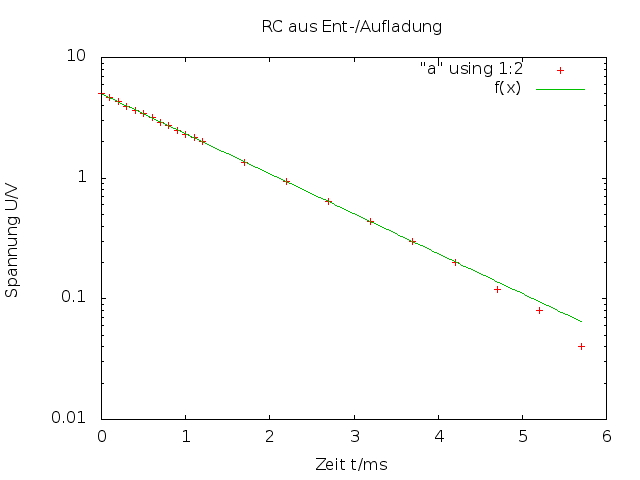
\includegraphics [width=0.7\textwidth] {pics/RC1.png}
\end{minipage}
\end{figure}
\begin{minipage}{0.2\textwidth}
\begin{tabular}{l|r}
$t/ms$ & $U/V$\\
\hline
0.0 &	5.00\\
0.1 &	4.62\\
0.2 &	4.32\\
0.3 &	3.96\\
0.4 &	3.66\\
0.5 &	3.42\\
0.6 &	3.16\\
0.7 &	2.92\\
0.8 &	2.72\\
0.9 &	2.50\\
1.0 &	2.32\\
1.1 &	2.16\\
1.2 &	2.00\\
1.7 &	1.36\\
2.2 &	0.94\\
2.7 &	0.64\\
3.2 &	0.44\\
3.7 &	0.30\\
4.2 &	0.30\\
4.7 &	0.12\\
5.2 &	0.08\\
5.7 &	0.04 
\end{tabular}
\end{minipage}



Die Steigung der Ausgleichsgeraden beläuft sich auf etwa $-7.62*10^2$. Somit ergibt sich für die Exponentialfunktion:

$U(t) = U_0 * exp(\frac{-t}{RC}) = 5V*exp(-7.62*10^{-2}s*t)$

\subsection{Frequenzabhängige Amplituden}
Indem das RC-Glied nun mit Sinusspannung höherer Frequenz betrieben wird, reicht die Periodendauer nicht aus, um 
den Kondensator komplett aufzuladen beziehungsweise zu entladen. Somit ergibt sich eine frequenzabhängige Amplitude der 
Kondensatorspannung, die entsprechend des oben aufgeführten Schaltbildes durch einen Millivoltmesser ermittelt wird. 
Die Generatorspannungsamplitude ist frequenzunabhängig bei U = 3.4 V. 

\begin{minipage}{0.2\textwidth}
\begin{tabular}{l|r}
$f/Hz$ & $A(\omega)/U_0$\\
\hline
0 &	1\\
10 &	0.64\\
50 &	0.6\\
100 &	0.49\\
150 &	0.4\\
200 &	0.33\\
250 &	0.27\\
300 &	0.23\\
350 &	0.20\\
400 &	0.18\\
500 &	0.14\\
600 &	0.12\\
700 &	0.100\\
800 &	0.098\\
900 &	0.074\\
1000 &	0.068\\
1200 &	0.053\\
1400 &	0.044\\
1600 &	0.038\\
1800 &	0.032\\
2000 &	0.024
\end{tabular}
\end{minipage}
\begin{figure}[htbp]
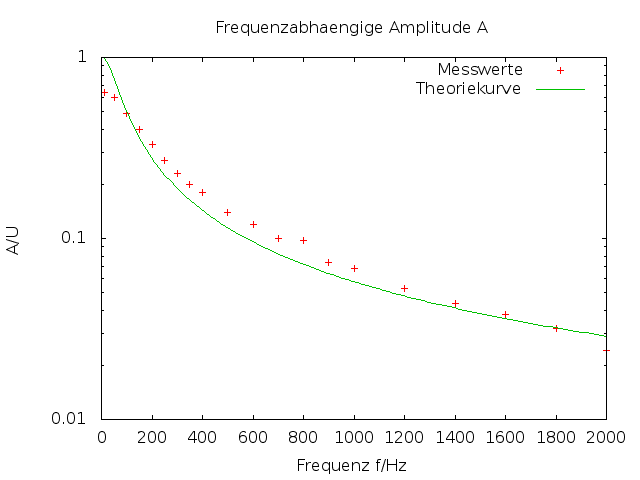
\includegraphics[width=8cm] {pics/RC2.png}
\centering
\end{figure}

Die Messwerte geben ein Verhältnis von $\frac{A(\omega)}{U}$, welches indirekt proportional zu $\omega$ ist. Die genaue
Abhängigkeit entspricht der aus Gleichung \eqref{A_omega} mit einem Wert für die Zeitkonstante RC von $2.76*10^{-3}s$. Somit
ist

\begin{align}
A(\omega)= \frac{5V}{\sqrt{1+\omega^2(2.76*10^{-3})^2}}
\notag
\end{align}

Dass der RC-Wert hier von dem unter 4.1 genannten abweicht, liegt an dem Innenwiderstand von $R_i = 600 \Omega$.

\subsection{Frequenzabhängige Phasenverschiebung}
Bei steigender Frequenz stellt sich eine Phasenverschiebung zwischen der Generatorspannung $U_0$ und der Kondensatorspannung 
$U_C$ ein. Dies läuft auf die Trägheit des RC-Gliedes hinaus, welche zunehmende Werte für $\phi$ hervorruft. Bei einem 
Zweistrahl-Oszilloskop wird der Generator am ersten Eingang und das RC-Glied am zweiten Eingang verbunden, sodass die Kathodenstrahlen
beider Sinusspannungen simultan angezeigt werden können.
\begin{figure}[htbp]
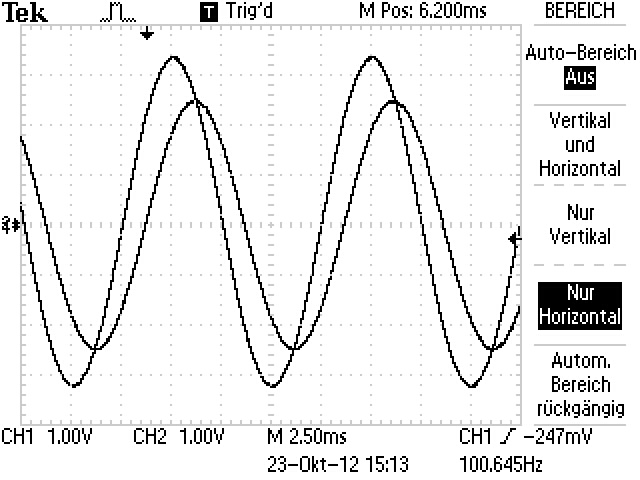
\includegraphics[width=8cm] {pics/Phi.JPG}
\centering
\end{figure}

Nun wird die zeitliche Differenz der Nulldurchläufe a beider Schwingungen, sowie ihre Periodendauer b ermittelt und aus ihnen
$\phi$ in Abhängigkeit der Frequenz der Kondensatorspannung bestimmt.

\begin{tabular}{l|r|r}
$f/Hz$ & $a/ms$	& $b/ms$\\
\hline
100 &	1.14 &	9.91\\
200 &	0.80 &	5.00\\
400 &	0.50 &	2.50\\
1000 &	0.23 &	1.00\\
2000 &	0.118 &	0.50
\end{tabular}
\begin{figure}[htbp]
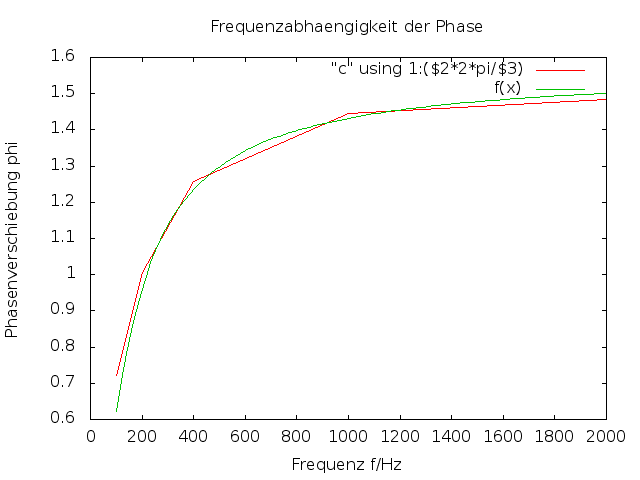
\includegraphics[width=8cm] {pics/RC3.png}
\centering
\end{figure}

Die von Gnuplot gefittete Ausgleichsfunktion $f(x)$ gibt als RC-Parameter $1.14*10^{-3}$ aus. Da diese Zahl in derselben
Größenordnung liegt, wie der richtige Wert der Zeitkonstanten, kann man diese Differenz damit erklären, dass die Funktion
nicht vollends die Kurve der Messpunkte beschreibt. $\phi$ ist proportional zum arcustangens von $\omega$. Für große Werte
von $\omega$ beeinflusst die Zeitkonstante das Ergebnis unerheblich und der arcustangens nähert sich $\frac{\pi}{2}$ an.

\subsection{RC-Glied als Integrator}
Bei gleichbleibender Schaltung soll nun mit dem Oszilloskop die Integrierfunktion des RC-Gliedes gezeigt werden. 
Hierzu werden vier verschiedene Spannungstypen angelegt und mit der Ausgabe des Kondensators verglichen. An den
Beispielen ist die Funktionsfähigkeit deutlich erkennbar.

\begin{figure}[htbp]
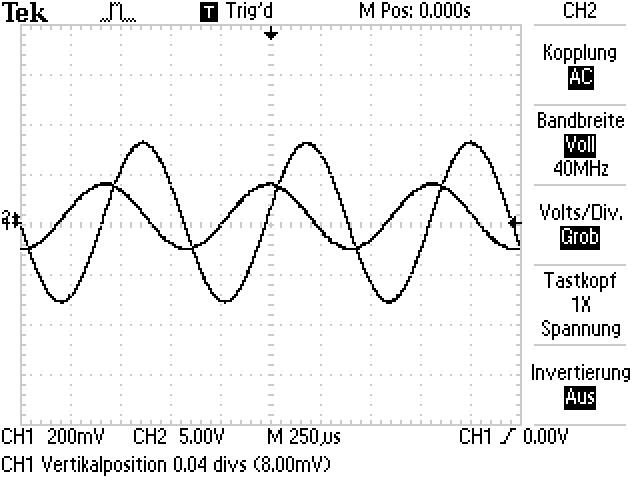
\includegraphics[width=8cm] {pics/sinus.JPG}
\centering
\caption{Sinus zu Cosinus}
\end{figure}

\begin{figure}[htbp]
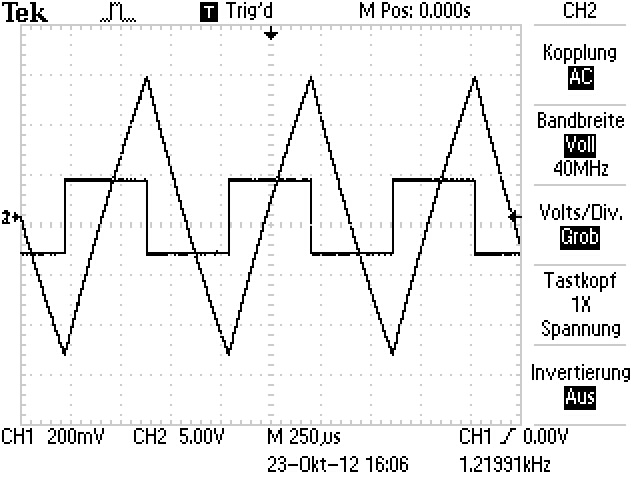
\includegraphics[width=8cm] {pics/rechteck2.JPG}
\centering
\caption{Rechteck zu Dreieck 1}
\end{figure}

\begin{figure}[htbp]
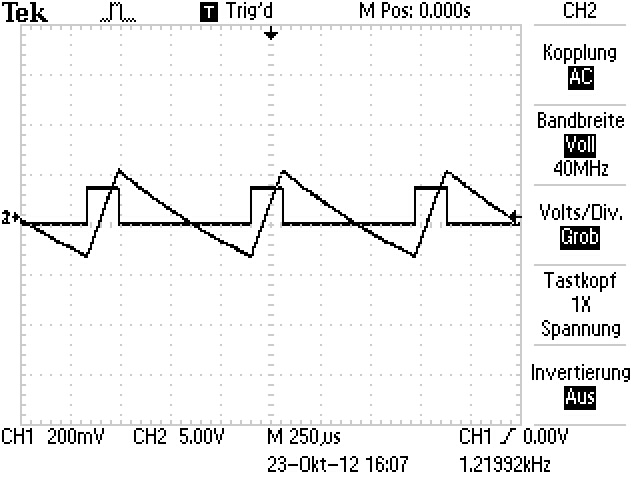
\includegraphics[width=8cm] {pics/rechteck1.JPG}
\centering
\caption* {Rechteck zu Dreieck 2}
\end{figure}

\begin{figure}[htbp]
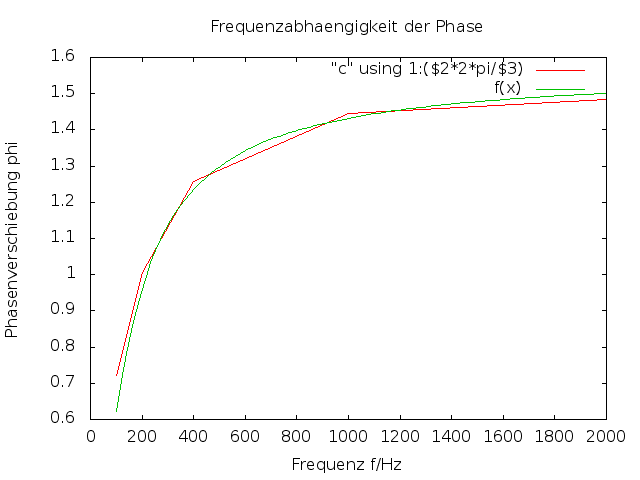
\includegraphics[width=8cm] {pics/RC3.png}
\centering
\end{figure}



% ========================================
%	Literaturverzeichnis
% ========================================

%\bibliographystyle{plainnat}			% Bibliographie-Style auswählen
%\bibliography{BIBDATEI}			% Literaturverzeichnis

% ========================================
%	Das Dokument endent
% ========================================

\end{document}
